


This preceding analysis demonstrates
several theoretical advantages 
to increasing impact parity via treatment disparity:
\begin{itemize}
\item \textbf{Optimality: } 
As demonstrated for CV score and for $p$-$\%$ rule, 
intervention via per-group thresholds 
maximizes accuracy subject to an impact parity constraint.
\item \textbf{Rational ordering:} Within each group, individuals with higher probability 
of belonging to the positive class
are always assigned to the positive class 
ahead of those with lower probabilities.
\item \textbf{Does no harm to the protected group:} The treatment disparity intervention 
can be constrained to only benefit members of the disadvantaged class.
\end{itemize}

% DLPs do not directly apply .
% To avoid treatment disparity,
DLPs attempt to produce a classifier 
that satisfies the parity constraints,
by relying upon the proxy features 
to satisfy the parity metric. 
Typically, this is accomplished 
either by introducing constraints 
to a convex optimization problem, 
or by adding a regularization term 
and tuning the corresponding hyper-parameter. 
Because the CV score and $p$-$\%$ rule 
are non-convex in model parameters 
(scores only change 
when a point crosses the decision boundary),
\cite{kamishima2011fairness, zafar2017fairness}
introduce convex surrogates 
aimed at reducing the correlation
between the sensitive feature and the prediction.

% ALEX: replacing "authors" with "approaches" so that the criticism is targeted at the methods not their creators.
These approaches presume that the proxy variables 
contain information about the sensitive attribute.
Otherwise, the parity could only be satisfied 
via a trivial solution 
(e.g.~assign either \emph{everyone} or \emph{nobody} 
to the positive class). 
So we must consider two scenarios: 
(i) the proxy variables $\mathbf{x}$ 
fully encode $z$,
in which case, a sufficiently powerful DLP 
will implicitly reconstruct $z$,
because this gives the optimal solution 
to the impact-constrained objective;
and (ii) $\vct x$ doesn't fully capture $z$, or the DLP is unable to recover $z$ from $\vct x$,
in which case the DLP may be sub-optimal,
may violate rational ordering within groups, 
and may harm members of the disadvantaged group.



%
%  ADDING THIS FUCKER BACK LET'S BE CAREFUL TO ADD ANY REFS IN INTO ETC SO IT'S NOT DROPPING OUT OF THE FUCKING SKY. 
% 
\subsection{Synthetic data example: work experience and hair length in hiring} \label{sec:synthetic}
To begin, we illustrate our arguments empirically 
with a simple synthetic data experiment.  
To construct the data, 
we sample $n_{\text{all}} = 2000$ total observations 
from the data-generating process described below.  
70\% of the observations are used for training, 
and the remaining 30\% are reserved for model testing.  
\begin{align*}
z_i &\sim \mathrm{Bernoulli}(0.5) \\
\mathrm{hair\_length}_i \mid z_i = 1 &\sim  35 \cdot \mathrm{Beta}(2,2) \\ 
\mathrm{hair\_length}_i \mid z_i = 0 &\sim  35 \cdot \mathrm{Beta}(2,7) \\ 
\mathrm{work\_exp}_i \mid z_i &\sim  \mathrm{Poisson}(25 + 6z_i) - \mathrm{Normal}(20, \sigma = 0.2) \\
y_i \mid \mathrm{work\_exp}  &\sim 2 \cdot \mathrm{Bernoulli}(p_i) - 1\text{,} \\ 
\text{where  } p_i &= 1 / \left(1 + \exp[-(-25.5 + 2.5\mathrm{work\_exp})]\right)
\end{align*}
This data-generating process 
has the following key properties: 
(i) the historical hiring process 
was based solely on the number of years of work experience; 
(ii) because women on average have fewer years of work experience than men (5 years vs. 11), 
men have been hired at a much higher rate than women; 
and (iii) women have longer hair than men, 
a fact that was irrelevant to historical hiring practice.

Figure \ref{fig:intragroup-disparity} 
shows the test set results of applying a DLP 
to the available historical data 
to equalize hiring rates between men and women.  
We apply the DLP proposed by \citet{zafar2017fairness}, 
using code available from the authors.\footnote{\url{https://github.com/mbilalzafar/fair-classification/}} 
While the DLP nearly equalizes hiring rates 
(satisfying a $105$-\% rule), 
it does so through a problematic 
within-class discrimination mechanism.  
The DLP rule advantages individuals 
with longer hair over those with shorter hair 
and considerably longer work experience.  
We find that several women 
who would have been hired under historical practices, 
owing to their 12+ years of work experience, 
would not be hired under the DLP 
due to their short hair 
(i.e., their male-like characteristics captured in $\vct x$). Similarly, several men,
who would not have been hired based on work experience alone, are advantaged by the DLP due to their longer hair  
(i.e., their `female-like' characteristics in $\vct x$).  
The DLP violates rational ordering, 
and harms some of the most qualified individuals 
in the protected group.  
Group parity is achieved at the cost of individual unfairness.  



Granted, we might not expect
factors such as hair length 
to knowingly be used as inputs 
to a typical hiring algorithm.  
% This example was constructed to
We construct this toy example to
illustrate a more general point:  
since DLPs do not have direct access 
to the protected feature, 
they must infer from the other features
which people are most likely to belong to each subgroup.  
Using the protected feature directly 
can yield more reasonable policies: 
For example, by applying per-group thresholds,
we could hire the highest rated individuals in each group, 
rather than distorting rankings within groups
based on how female/male individuals \emph{appear} 
to be from their other features.

\begin{figure*}[t]
\begin{center}
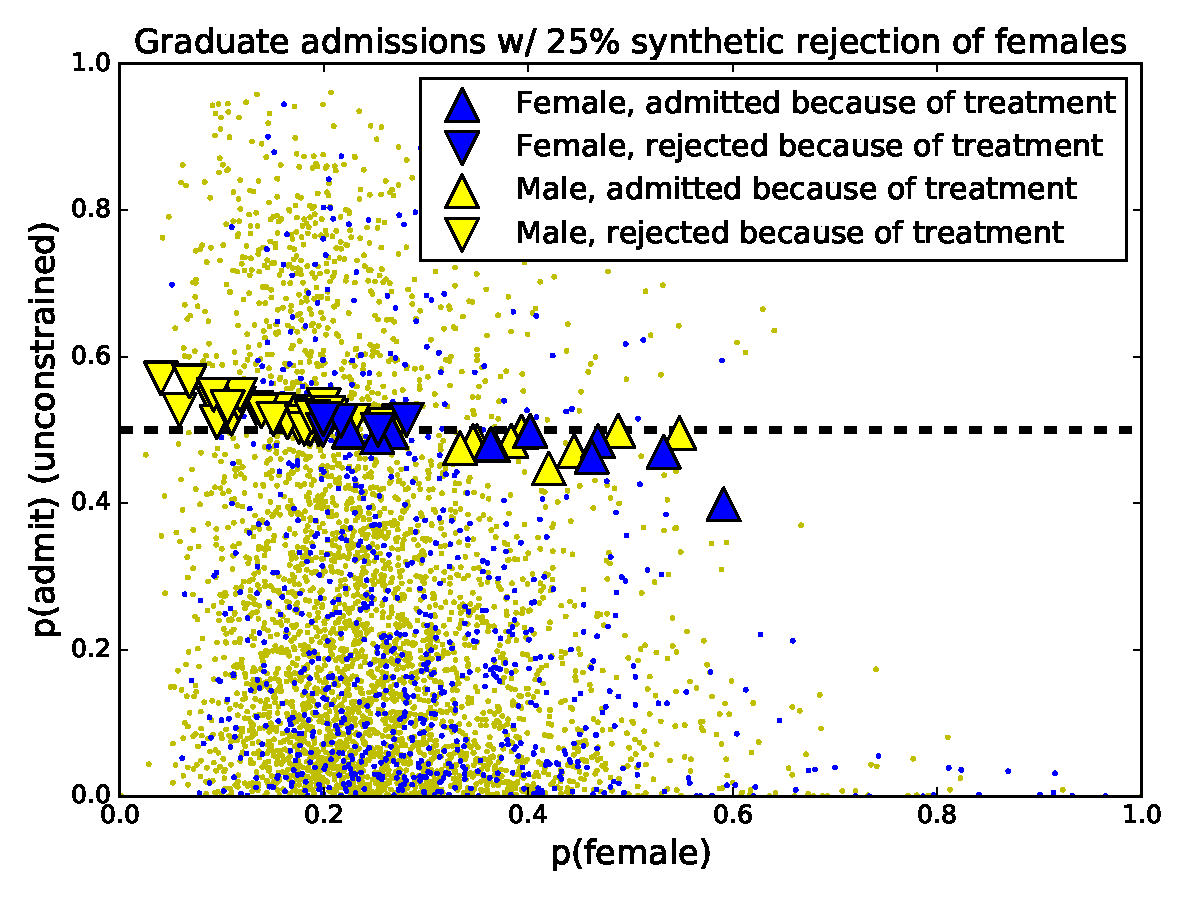
\includegraphics[width=0.33\linewidth]{img/plot_zoomedout}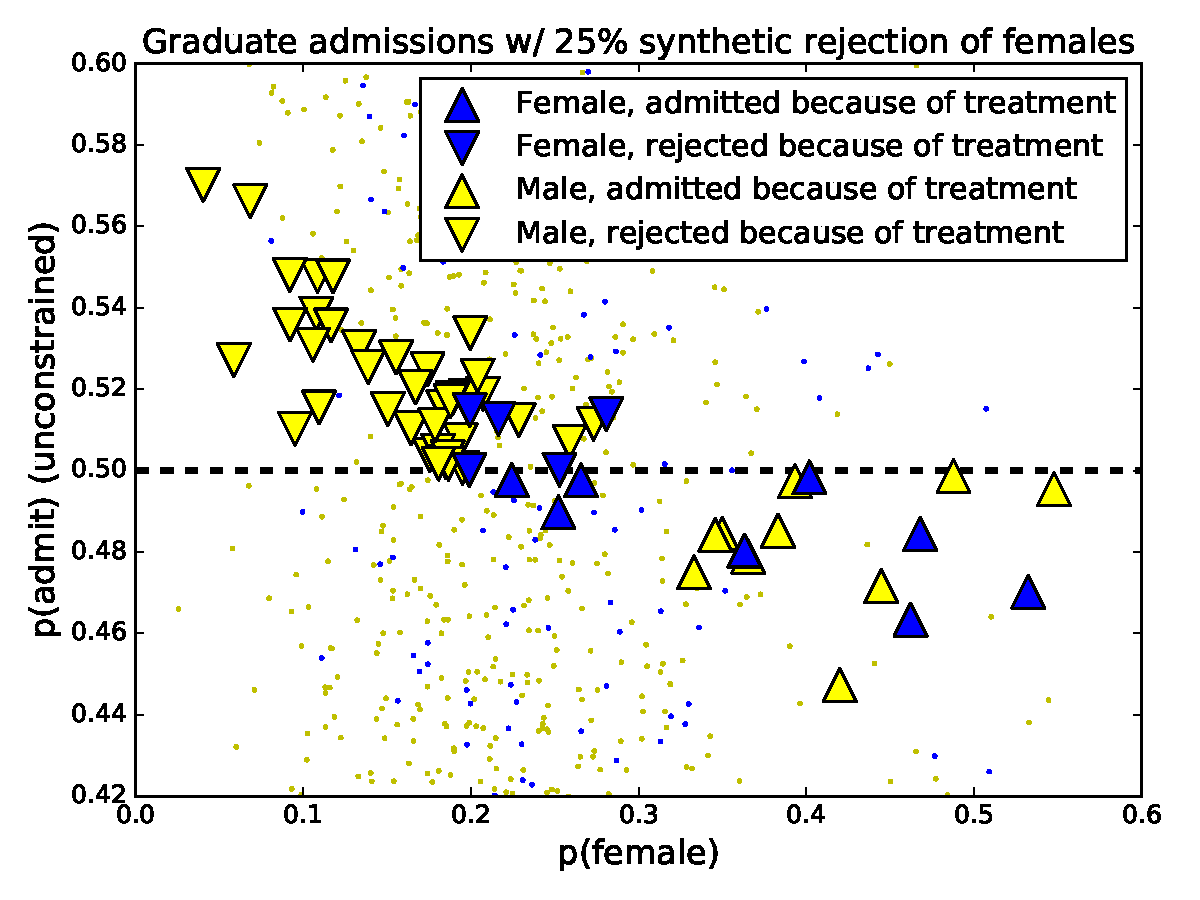
\includegraphics[width=0.33\linewidth]{img/plot}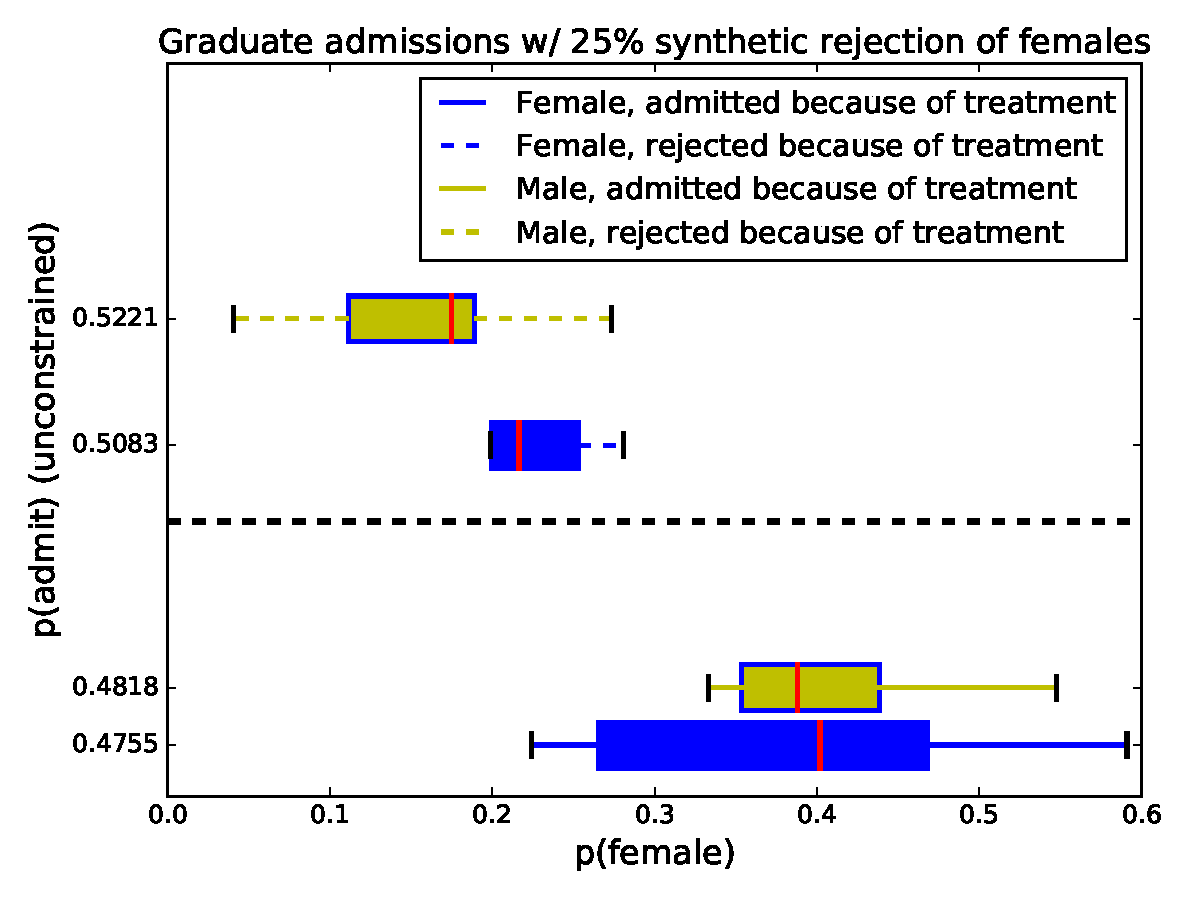
\includegraphics[width=0.33\linewidth]{img/whisker}
\end{center}
\caption{
(left) probability of the sensitive variable 
versus (unconstrained) admission probability, 
on unseen test data. 
%  above 0.5 
Downward triangles indicate individuals 
rejected
\emph{only} after applying the DLP (``treatment''), 
while upward triangles indicate individuals 
accepted \emph{only} by the DLP.
The remaining $\sim$4,000 blue/yellow dots
indicate people whose decisions are not altered. 
Many students benefiting from the DLP 
are males who `look like' females based on other features, 
whereas females who `look like' males are hurt by the DLP. Detail view (center) and summary statistics (right) of the same plot.}
\label{fig:admissions}
\end{figure*}

% \vspace{-0.5em}

\subsection{Case study: Gender bias in CS graduate admissions}
\label{sec:admissions}
\label{sec:threshold}

% \vspace{-1em}

For our next example,
we demonstrate a similar result 
but this time by analyzing real data 
%We first consider a real dataset, 
with synthetic discrimination, to empirically demonstrate our arguments.
We consider a sample of $\sim$9,000 students 
considered for admission 
to the MS program 
of a large US university
over an 11-year period.
%(2006-2016). 
Half of the examples are withheld for testing. 
Available attributes include
basic information, 
such as country of origin, interest areas, 
and gender, 
as well as quantitative fields 
such as GRE scores. 
Our data also includes a label 
in the form of an `above-the-bar' decision 
provided by faculty reviewers.
%\footnote{
% These decisions do not precisely determine 
% whether a student is made an offer, 
% but rather represent an `above-the-bar' assessment 
% that is used to guide admissions decisions,
% and can be considered as a binary label.}
%
Admission rates for male and female applicants 
were observed to be within 1\% of each other.
So, to demonstrate the effects of DLPs, 
we corrupt the data with \emph{synthetic discrimination}.
Of all women who were admitted, i.e., $z_i = b, y_i = 1$,
we flip 25\% of those labels to $0$:
giving noisy labels $\bar{y}_i = y_i \cdot \eta$, 
for $\eta \sim \textit{Bernoulli}(.25)$.
This simulates %a setting in which 
%the training data exhibits a historical bias.
historical bias in the training data.

We then train three logistic regressors: 
(1) To predict the (synthetically corrupted) labels $\bar y_i$
from the non-sensitive features 
$x_i$; 
(2) The same model, applying the DLP of \citep{zafar2017fairness}; and 
(3) A model 
to predict the sensitive feature  $z_i$
from the non-sensitive features $x_i$. 
The data contains limited information 
that predicts gender, 
though such predictions can be made better 
than random (AUC=0.59) 
due to different rates of gender imbalance 
across (e.g.)~countries and interests.

%JULIAN: Note that my unconstrained classifier does not use the sensitive variable for prediction.

% To shape our intuition for what is happening here, we also train a classifier to predict $z$ given $z_i$. 

Figure~\ref{fig:admissions} (left) shapes 
our basic intuition for what is happening:
Considering the probability of admission 
for the unconstrained classifier (y-axis), 
students whose decisions are `flipped' 
(after applying the fairness constraint)
tend to be those close to the decision boundary. 
Furthermore, students \emph{predicted} to be male (x-axis)
tend to be flipped to the negative class 
(left half of plot) 
while students \emph{predicted} to be female 
tend to be flipped to the positive class 
(right half of plot). 
This is shown in detail 
in Figure~\ref{fig:admissions} (center and right). 
Of the 43 students whose decisions are flipped to `non-admit,' 5 are female, 
each of whom has `male-like' characteristics 
according to their other features
as demonstrated in our synthetic hair-length example.
Demonstrated here with real-world data,
% Here
the DLP both disrupts the within-group ordering
and violates the \emph{do no harm} principle 
by disadvantaging some women who, but for the DLP, 
would have been admitted. 

% \julian{Add some take-home to the above. Also, fix the p-rule stuff below to match your notation.}
\paragraph{Comparison with Treatment Disparity.}
% \label{sec:threshold}
To demonstrate the better performance 
of per-group thresholding, 
%(violating treatment parity), 
we implement a simple decision scheme
and compare its performance to the DLP.


Our thresholding rule
for maximizing accuracy 
subject to a $p$-$\%$ rule works as follows:
Recall that the $p$-$\%$ rule requires 
that $q_b/q_a > p/100$, which can be written as
$\frac{p}{100} q_a - q_b < 0$.
We denote the quantity $\frac{p}{100} q_a - q_b$ as the $p$-gap.
To maximize accuracy subject to satisfying the $p$-$\%$ rule,
we construct a score
that quantifies reduction in $p$-gap 
per reduction in accuracy.
Starting from the accuracy-maximizing classifications $\hat y$
(thresholding at $.5$),
we then flip those predictions 
which close the gap fastest:



\begin{enumerate}
\item Assign each example with $\lbrace \tilde{y}_i =0, z_i=b\rbrace$ or $\lbrace\tilde{y}_i = 1, z_i=a \rbrace$,
a score $c_i$ 
equal to the reduction in the p-gap 
divided by the reduction in accuracy:
\begin{enumerate}
\item For each example in group $a$ with initial $\hat{y}_i=1$,
$c_i = \frac{p}{100n_a(2\hat{p}_i-1)}$.
\item For each example in group $b$ with initial $\hat{y}_i=0$,
$c_i = \frac{1}{n_b(1-2\hat{p}_i)}$.\\[-0.5\baselineskip]
\end{enumerate}
\item Flip examples in descending order 
according to this score 
until the desired CV-score is reached.
\end{enumerate}
These scores do not change after each iteration, so the greedy policy leads to optimal flips (equivalently, optimal classification thresholds).


% \begin{wraptable}{r}{.5\linewidth}
\begin{table}
\centering
% \vspace{-0.5\baselineskip}
\caption{Statistics of public datasets.\label{tab:datastats}}
\footnotesize 
% \vspace{-2mm}
% \setlength{\tabcolsep}{2.25pt}
\begin{tabular}{llllr}
\toprule
\textbf{dataset} & \textbf{source} & \textbf{protected feature} & \textbf{prediction target} & $n$ \\
\midrule
Income & UCI \citep{uci_income} & Gender (female) & income $>$ \$50k & 32,561\\
Marketing & UCI \citep{uci_marketing} & Status (married) & customer subscribes & 45,211\\
Credit & UCI \citep{uci_default} & Gender (female) & credit card default & 30,000\\
Employee Attr. & IBM \citep{ibm_data} & Status (married) & employee attrition & 1,470\\
Customer Attr. & IBM \citep{ibm_data} & Status (married) & customer attrition & 7,043\\
\bottomrule
\end{tabular}
\normalsize
% \vspace{-3mm}
% \setlength{\tabcolsep}{6pt}
% \vspace{-0.5\baselineskip}
\end{table}
% \end{wraptable}

The unconstrained classifier achieves a p-\% rule of 71.4\%.  By applying this thresholding strategy, 
we were able to obtain the same accuracy 
as the method of \cite{zafar2017fairness}, 
but with a higher $p$-\% rule of 78.3\% compared to 77.6\%.  Note that on this data, the method of \cite{zafar2017fairness} maxes out at a $p$-\% rule of 77.6\%.  That is, the method is limited in what $p$-\% rules may be achieved.  By contrast, the thresholding rule can achieve any desired parity level.  Subject to a $<1\%$ drop in accuracy relative to the DLP we can achieve a $p$-\% rule of $\sim{}100$\%.
% Similarly, we could achieve a modest improvement in accuracy (<0.1\%) 
% while maintaining the same $p$-\% rule as the method of \cite{zafar2017fairness}.

% This example reveals that the method
% of \cite{zafar2017fairness}
% cannot produce any specified $p$-\%-rule. 
% On this data
% their algorithm maxes out at a $p$-\% rule of 77.59\%, 
% compared to a $p$-\% rule of 71.44\% 
% by na\"ive classification (on unseen test data). 
% Both have similar accuracy: 
% given that both positive labels 
% and female applicants are a minority, 
% assigning negative labels to males 
% close to the boundary impacts accuracy very little. 
% Both methods had accuracy of around 78\% on this data.
% Critically though, 
% by applying an optimal thresholding strategy, 
% we were able to obtain the same accuracy 
% as the method of \cite{zafar2017fairness}, 
% but with a higher $p$-\% rule of 78.34\%; subject to a $<1\%$ drop in accuracy we can achieve a $p$-\% rule of $\sim{}100$\%.
% Similarly, we could achieve a modest improvement in accuracy (<0.1\%) 
% while maintaining the same $p$-\% rule as the method of \cite{zafar2017fairness}.

% \vspace{-0.5em}

\subsection{Examples on public datasets}

% \vspace{-0.5em}

Finally, for reproducibility,
we repeat our experiments from Section \ref{sec:admissions}
on a variety of public datasets (code and data will be released at publication time).
%\footnote{Code and data available on \url{http://jmcauley.ucsd.edu/code/fairness/}}
Again we compare applying our simple thresholding scheme against the fairness constraint of \cite{zafar2017fairness}, considering a binary outcome 
and a single protected feature. 
Basic info about these datasets 
(including the prediction target and protected feature) 
is shown in Table~\ref{tab:datastats}.


The protocol we follow is the same as in Section \ref{sec:admissions}. 
Each of these datasets exhibits a certain degree of bias 
w.r.t.~the protected characteristic (Table~\ref{tab:results}), 
so no synthetic discrimination is applied. 
In Table~\ref{tab:results},
we compare (1) The $p$-\% rule obtained 
using the classifier of \cite{zafar2017fairness} 
compared to that of a na\"ive classifier 
(column k vs.~column h); and 
(2) The $p$-\% rule obtained 
when applying our thresholding strategy 
from Section~\ref{sec:threshold}.
As before, half of the data are withheld for testing.

First, we note that in most cases, 
the method of \cite{zafar2017fairness} increases 
the $p$-\% rule (column k vs.~h),
while maintaining an accuracy similar 
to that of unconstrained classification (column i vs.~f). 
One exception is the UCI-Credit dataset, 
in which \emph{both} the accuracy 
and the $p$-\% rule simultaneously decrease; 
although this is against our expectations, 
note that the optimization technique of \cite{zafar2017fairness} is an approximation scheme 
and does not offer accuracy guarantees in practice (nor can it in general achieve a $p$-\% rule of 100\%). 
However these details are implementation-specific 
and not the focus of this paper.
%
Second, as in Section~\ref{sec:threshold}, 
we note that the optimal thresholding strategy 
is able to offer a strictly larger $p$-\% rule 
(column l vs. k) at a given accuracy 
(in this case, the accuracy from column i). 
In most cases, we can obtain a $p$-\% rule 
of (close to) 100\% at the given accuracy.

\begin{table*}[t!]
\centering
\caption{Comparison between unconstrained classification, DLPs, and thresholding schemes.
Note that the $p$-\% rules from \cite{zafar2017fairness} were the strongest that could be obtained with their method; 
on complex datasets $p$-\% rules of 100\% 
are rarely obtained in practice, 
due to their specific approximation scheme.
Employee and Customer datasets are from IBM, the others are UCI datasets.
\label{tab:results}}
\scriptsize
\setlength{\tabcolsep}{3pt}
\begin{tabular}{lcccc|ccr|ccr|r}
\toprule
\multicolumn{5}{c|}{\textbf{basic statistics}} & \multicolumn{3}{c|}{\parbox{0.17\textwidth}{\centering \textbf{na\"ive (unconstrained)\\ classification}}} & \multicolumn{3}{c|}{\parbox{0.17\textwidth}{\centering \textbf{fair (constrained)\\ classification \citep{zafar2017fairness}}}} & \multicolumn{1}{c}{\parbox{0.08\textwidth}{\centering \textbf{optimal\\ threshold}}} \\
\midrule
\multicolumn{1}{c}{\textbf{dataset}} & \textbf{\%prot.} & 
\parbox{0.06\textwidth}{\centering \textbf{\%prot.\\ in +'ve}} & \parbox{0.09\textwidth}{\centering \textbf{\%non-prot.\\ in +'ve}} & \textbf{label $p$-\%} & \textbf{acc.} & \parbox{0.11\textwidth}{\centering \textbf{prot./non-prot.\\ in positive}} & \textbf{$p$-\%} & \textbf{acc.} & \parbox{0.11\textwidth}{\centering \textbf{prot./non-prot.\\ in positive}} & \textbf{$p$-\%} & \parbox{0.11\textwidth}{\centering \textbf{$p$-\% at\\ const.~acc.}}\\[1mm]
\multicolumn{1}{c}{a} & b & c & d & e & f & g & \multicolumn{1}{c|}{h} & i & j & \multicolumn{1}{c|}{k} & \multicolumn{1}{c}{l}\\
\midrule
Income    & 66.9\% & 30.6\% & 10.9\% & 35.8\% & 0.85 & \ 8\% / 25\% & 31\% & 0.85 & \ 7\% / 24\% & 29\% & 52.9\% \\
Marketing & 60.2\% & 14.1\% & 10.1\% & 71.9\% & 0.89 & \ 3\% / \ 4\% & 82\% & 0.89 & \ 3\% / \ 3\% & 102\% & 100.3\% \\
Credit    & 60.4\% & 24.1\% & 20.8\% & 86.0\% & 0.82 & 10\% / 12\% & 88\% & 0.74 & 21\% / 25\% & 85\% & 100.0\% \\
Employee  & 45.8\% & 19.2\% & 12.5\% & 65.0\% & 0.87 & \ 8\% / 12\% & 65\% & 0.86 & \ 8\% / 11\% & 69\% & 100.4\%\\
Customer  & 48.3\% & 33.0\% & 19.7\% & 59.7\% & 0.80 & 15\% / 30\% & 49\% & 0.79 & 16\% / 19\% & 84\% & 100.2\%\\
\bottomrule
\end{tabular}
\normalsize
\setlength{\tabcolsep}{6pt}
\end{table*}

We emphasize that the goal of our experiments 
is not to `beat' the method of \citep{zafar2017fairness}, 
or even to comment on any specific discrimination-aware classification scheme. 
Rather, we emphasize that \emph{any} DLP
is fundamentally upper-bounded 
(in terms of the $p$-\% rule/accuracy trade-off) 
by simple schemes that explicitly consider the protected feature. 
% Not only do o
Our experiments validate this claim, 
and reveal that %that the practical difference 
% between the two schemes is significant: 
the two schemes make strikingly different decisions. 
While concealing the protected feature 
from the classifier may be conceptually desirable, 
% practitioners of such schemes 
practitioners should be aware of the consequences. 
% of doing so.
